\documentclass{article}
\usepackage[english]{babel}
\usepackage[letterpaper,top=2cm,bottom=2cm,left=3cm,right=3cm,marginparwidth=1.75cm]{geometry}
\usepackage{bm, amsmath, amssymb, enumerate, graphicx, float, booktabs, subfloat, subfig, caption, array}
\usepackage[ruled,linesnumbered]{algorithm2e}
\usepackage[hidelinks]{hyperref}

\title{\textbf{CS303 Artifitial Intelligence 2024F Project2 Report}}
\author{Ben Chen \\ \texttt{chenb2022@mail.sustech.edu.cn}}

\begin{document}
\maketitle

\section{Subtask 1 Supervised Learning}

\subsection{Introduction}

Unlike the previous project, this project introduces us to the world of machine learning through the lens of supervised learning. In this subtask, we are required to solve the problem of predicting the labels of the test data based on the training data.

More specifically, given a vectorized figures, we need implement a \texttt{Classifier} class along with a model, and train the model on the data. The data is accompanied by a set of labels, instead of a binary label, to indicate their kind. The model should be able to predict the labels of the test data.

\subsection{Methodology}

Intuitively, the multi-class classification problem can be solved by \textit{Softmax Regression} as described in \href{alg:softmax-fit}{Fit} and \href{alg:softmax-infer}{Inference}. Before that, some data preprocessing should be done:
\begin{enumerate}
    \item \textbf{Pruning} Remove the index column from training data/labels and test data/labels since it's not useful for classification and might misguide the model.
    \item \textbf{Normalization} The Softmax model requires the input data to be normalized, so we transform the distribution from $X \sim N(\mu, \sigma)$ to $Z \sim N(0, 1)$ with $Z = (X - \mu) / {\sigma}$.
    \item \textbf{One-hot Encoding} The labels are represented by integers, so we need to convert them to one-hot encoding vectors.
    \item \textbf{Data Splitting} Split the training data into training and validation data to evaluate the model, as learnt from the lab session.
\end{enumerate}

Softmax Regression is a generalization of Logistic Regression to the case where we want to handle multiple classes. In Softmax Regression, for input $\{(X_0, y_0), (X_1, y_1), \cdots, (X_m, y_m)\}$ with $k$ classes, the probabilities of the sample $X$ belonging to every classes is:

\[
    P(X; W) = \frac{1}{\sum_{j=1}^{k} e^{W_j^T X}} \begin{bmatrix}
        e^{W_1^T X} \\
        e^{W_2^T X} \\
        \vdots \\
        e^{W_k^T X}
    \end{bmatrix}
\]

so the probability of $X$ belonging to class $i$ is

$$
P(y = i | X; W) = \frac{e^{W_i^T X}}{\sum_{j=1}^{k} e^{W_j^T X}}
$$

The loss function of Softmax Regression is defined as:
\[
    L(W) = -\frac{1}{N} \sum_{i=1}^{N} \sum_{k=1}^{K} 1\{y_i = k\} \log \frac{e^{W_k^T x_i}}{\sum_{j=1}^{K} e^{W_j^T x_i}},\quad 
    W = \begin{bmatrix}
        w_1^T \\
        w_2^T \\
        \vdots \\
        w_K^T
    \end{bmatrix}
\]
where $W$ is the coefficient matrix of the model. And to maximize the likelihood, we solve the optimization problem by gradient descent:

\[
    \nabla_{w_k} L(W) = -\frac{1}{N} \sum_{i=1}^{N} x_i (1\{y_i = k\} - P(y = k | x_i; W))
\]

We can implement the algorithm with pseudo code in \href{alg:softmax-fit}{Softmax Fit} and \href{alg:softmax-infer}{Softmax Inference} below.

\begin{algorithm}
\caption{Softmax Regression Fit}\label{alg:softmax-fit}
\KwData{Training data $X\_train$, training labels $y\_train$, test data $X\_val$, test labels $y\_val$, $num\_iteration$, $learning\_rate$}
\KwResult{Model $W$, losses $L$ and accuracies $A$}

$L_X, L_y, A_X, A_y \leftarrow \textit{empty set}$ \;
$X\_train\_bias \leftarrow \textit{Randomly add bias to }X\_train$ \;
$weights \leftarrow \textit{Randomly initialize weights with} \dim(X) \times k$ \;
$k \leftarrow \text{Number of labels}$ \;
$m \leftarrow \text{Number of training samples}$ \;
$\mu \leftarrow \text{Mean of }X\_train$ \;
$\sigma \leftarrow \text{Standard deviation of }X\_train$ \;

\ForEach{iteration $i: 1 \to num\_iteration$}{
    $exp\_logits \leftarrow e^{X\_train\_bias \cdot weights}$ \;
    $prob \leftarrow exp\_logits / \sum_j exp\_logits_{1, j}$ \;
    $loss \leftarrow -\text{mean}(y\_train \cdot \log(prob))$ \;
    $gradient \leftarrow X\_train\_bias^T \cdot (prob - y\_train) / m$\;
    $weights \leftarrow weights - \text{learning\_rate} \cdot gradient$\;
    $L_X \leftarrow L_X \cup \{loss\}$\;
    $A_X \leftarrow A_X \cup \{\text{accuracy}(prob, y\_train)\}$\;

    $X\_val\_bias \gets$ concatenate a column of ones to $X\_val$ \;
    $logits\_val \gets X\_val\_bias \cdot weights$ \;
    $exp\_logits\_val \gets$ element-wise exponential of $logits\_val$ \;
    $probs\_val \gets exp\_logits\_val /$ sum of $exp\_logits\_val$ along axis 1 (keepdims=True) \;
    $val\_loss \gets -$ mean of element-wise product of $y\_val$ and $\log(probs\_val)$ \;
    $val\_pred \gets$ index of maximum value in $probs\_val$ along axis 1 \;
    $val\_accuracy \gets$ mean of $(val\_pred ==$ index of maximum value in $y\_val$ along axis 1) \;
    
    $L_y \leftarrow L_y \cup \{val\_loss\}$\;
    $A_y \leftarrow A_y \cup \{val\_accuracy\}$\;
}
\Return $W=\{weights, k, \mu, \sigma\}, L=\{L_X, L_y\}, A=\{A_X, A_y\}$\;
\end{algorithm}

And in inference process, we pick the label with the maximum probability as the predicted label:

\begin{algorithm}
\caption{Softmax Regression Inference}\label{alg:softmax-infer}
\KwData{Vectorized figure $X$, model $W$}
\KwResult{Predicted label $y$}
$X \leftarrow (X - \mu) / \sigma$ \;
$bias \leftarrow \text{Concatenate a column of ones to }X$ \;
$y \leftarrow \text{Label of maximum value in }(bias \cdot weights),\ weights \in W$ \;
\Return $y$\;
\end{algorithm}

\paragraph{Comlexity Analysis} In training process, the time cost of each iteration is $O(\dim(X) \cdot m \cdot k)$, where $m$ is the number of training samples and $k$ is the number of labels, since the most time-consuming calculation is the cross-entropy loss. In inference process, the time cost is $O(k\cdot m)$ for the matrix multiplication. The overall space complexity is $O(\dim(X) \cdot k \cdot m)$ for the input data and weights.

\paragraph{Hyperparameters} Totally we can tune four of the coefficients in the model, which are
\begin{enumerate}
    \item \textbf{Learning Rate} The step size of the gradient descent algorithm.
    \item \textbf{Number of Iteration} The number of iterations to train the model. It's trivial to the training process since the model will converge after a certain number of iterations. So it only affects the training time.
    \item \textbf{Seed} The random seed for the random initialization of the weights. This will affect the selection of training data and validation data, and the initialization of the weights.
    \item \textbf{Ratio of Training Data} The ratio of splitting the training data into training and validation data. It's said that 0.7 or 0.8 is good enough.
\end{enumerate}
So we largely adjust the learning rate and evaluate the accuracy with test dataset, while we will ensure that the model is trained with enough iterations.

\subsection{Experiments}

\subsubsection{Metrics}

In experiments of this subtask, we adapt a compound testing methods to evaluate the effectiveness of the algorithms, which is to train the model locally and test remotely. For local testing, we use the following environment:
\begin{table}[!htbp]
    \begin{center}
    \begin{tabular}[c]{cc}
        \textbf{Model} & MacBook Air M3 13' \\
        \textbf{CPU} & Apple M3 4E + 4P 2.4GHz-3.7GHz \\
        \textbf{Memory} & LPDDR5-6400 8GB Unified Memory
    \end{tabular}
    \end{center}
\end{table}

And for remote testing, we use the following environment:

\begin{table}[!htbp]
    \begin{center}
    \begin{tabular}[c]{cc}
        \textbf{Model} & Online Judge \\
        \textbf{CPU} & Intel Xeon E5-2680 2.2GHz * 1 \\
        \textbf{Memory} & 3GB DDR4 2666MHz
    \end{tabular}
    \end{center}
\end{table}

We tested the training cost on the local environment and the accuracy on the remote environment, with different parameters mentioned above. For training, we utilize the \texttt{image\_classification.ipynb} to visualize the loss and accuracy during training. For testing, we recorded the accuracy of the model on the test dataset that evaluated by the online judge.

\subsubsection{Results}

The loss and accuracy diagrams are shown below:

\begin{figure}[htbp]
  \centering
  \subfloat[Accuracy of training]
  {
      \label{fig:acc-1}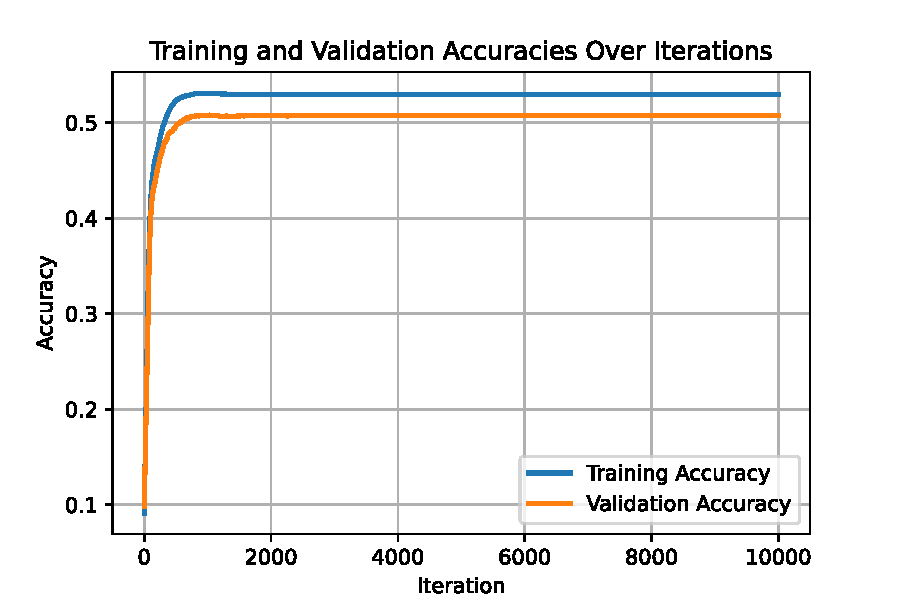
\includegraphics[width=0.4\textwidth]{img/softmax-acc-1.pdf}
  }
  \subfloat[Loss of training]
  {
      \label{fig:loss-1}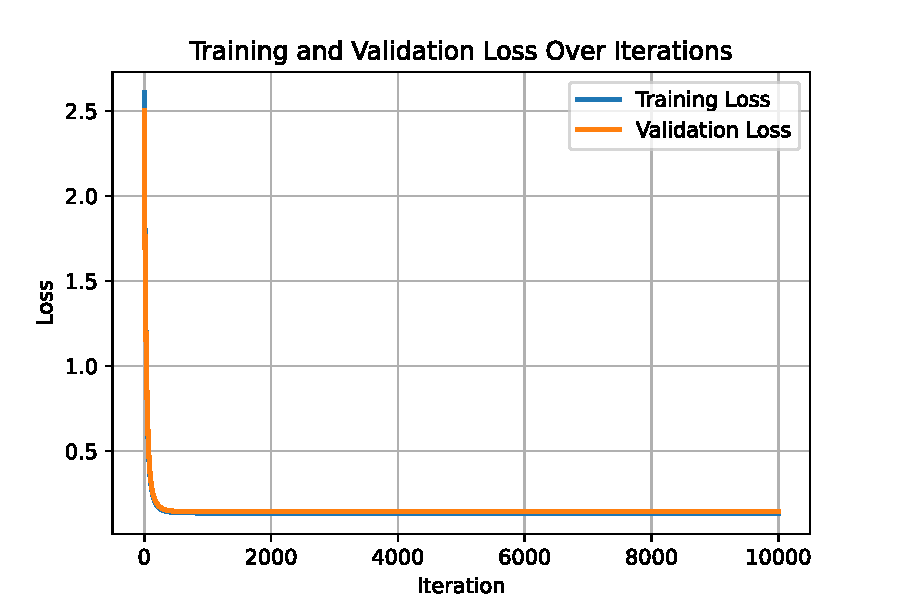
\includegraphics[width=0.4\textwidth]{img/softmax-loss-1.pdf}
  }
  \caption{Softmax Regression with Learning Rate = 1}
\end{figure}

\begin{figure}[htbp]
  \centering
  \subfloat[Accuracy of training]
  {
      \label{fig:acc-0.1}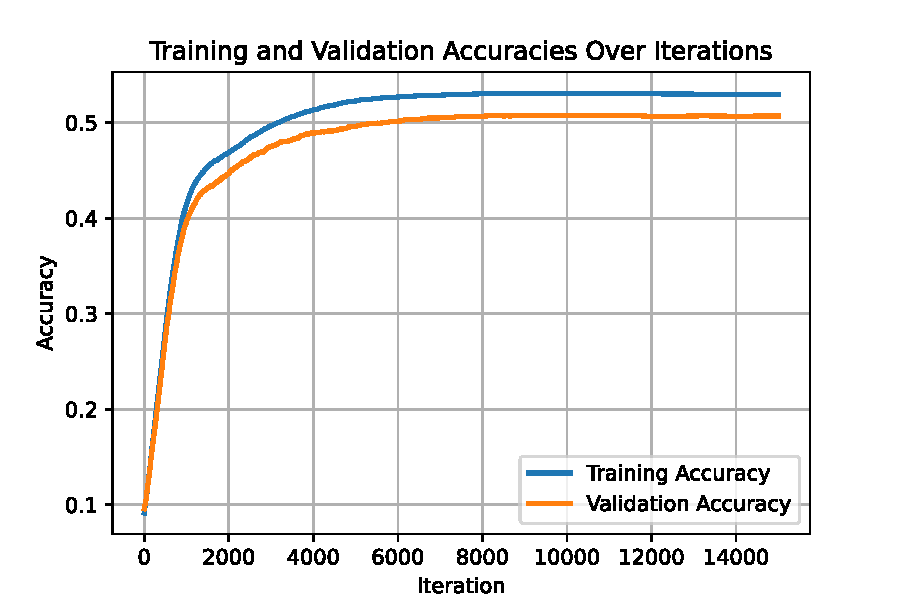
\includegraphics[width=0.4\textwidth]{img/softmax-acc-0.1.pdf}
  }
  \subfloat[Loss of training]
  {
      \label{fig:loss-0.1}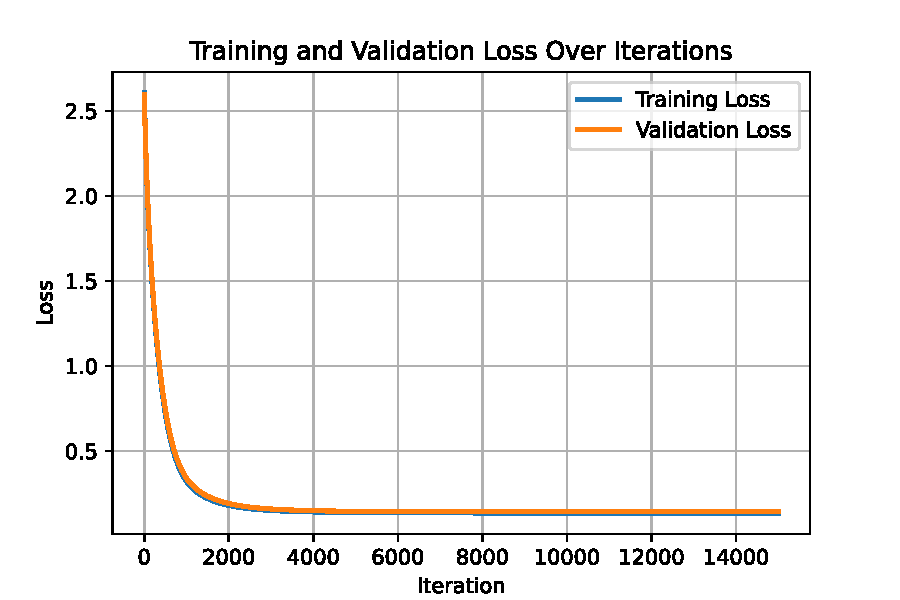
\includegraphics[width=0.4\textwidth]{img/softmax-loss-0.1.pdf}
  }
  \caption{Softmax Regression with Learning Rate = 0.1}
\end{figure}

\begin{figure}[htbp]
  \centering
  \subfloat[Accuracy of training]
  {
      \label{fig:acc-0.05}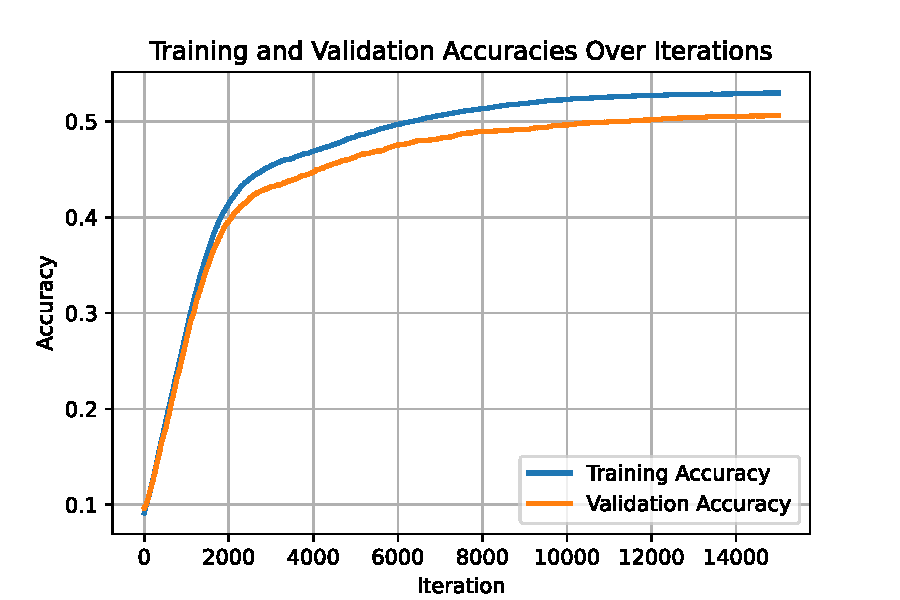
\includegraphics[width=0.4\textwidth]{img/softmax-acc-0.05.pdf}
  }
  \subfloat[Loss of training]
  {
      \label{fig:loss-0.05}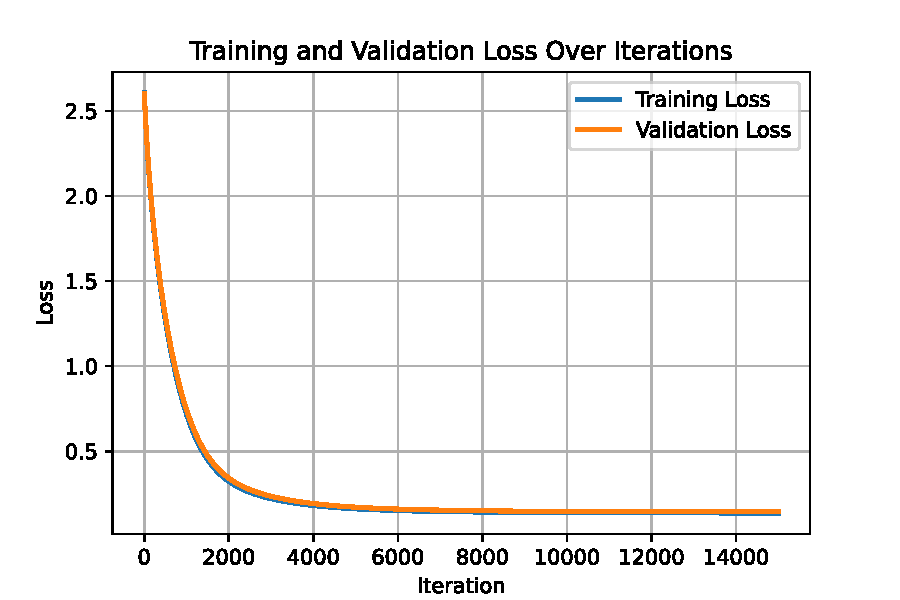
\includegraphics[width=0.4\textwidth]{img/softmax-loss-0.05.pdf}
  }
  \caption{Softmax Regression with Learning Rate = 0.05}
\end{figure}

\begin{figure}[htbp]
  \centering
  \subfloat[Accuracy of training]
  {
      \label{fig:acc-0.002}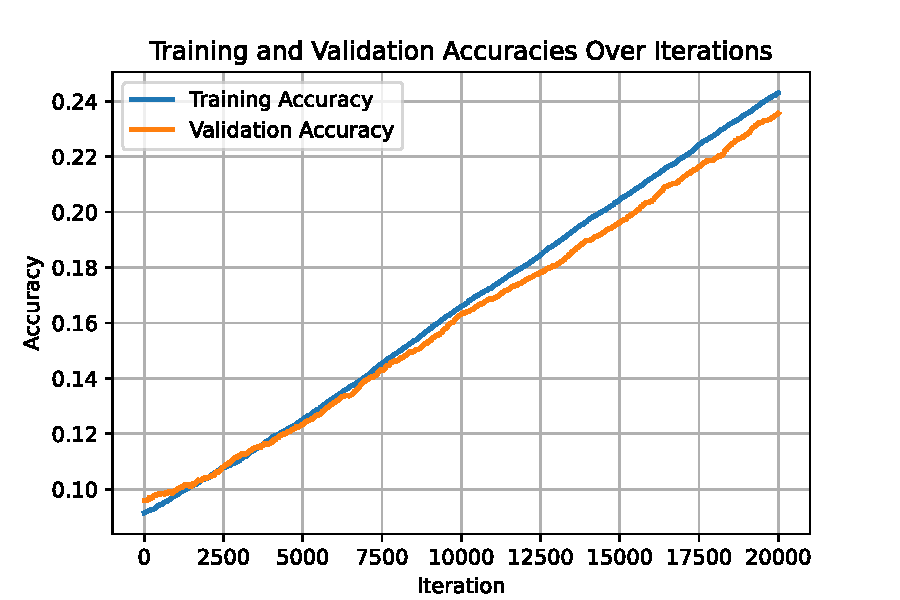
\includegraphics[width=0.4\textwidth]{img/softmax-acc-0.002.pdf}
  }
  \subfloat[Loss of training]
  {
      \label{fig:loss-0.002}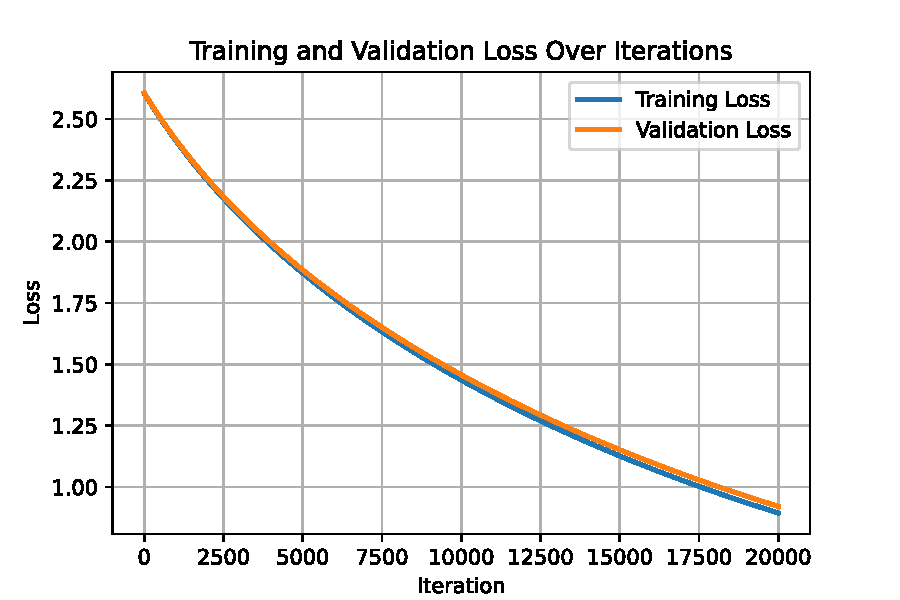
\includegraphics[width=0.4\textwidth]{img/softmax-loss-0.002.pdf}
  }
  \caption{Softmax Regression with Learning Rate = 0.002}
\end{figure}

As we can tell from the above figures, the accuracies are quite closed to each other when converging with LR = 1, 0.1, 0.05. However, when LR = 0.002, the learning speed dropped significantly and did not converge within 20000 iterations. Also from the accuracy and loss diagram, the both converge faster with higher learning rate and slower with lower learning rate, while the difference between training and validation accuracy remains similar.

\begin{table}[!htbp]
\setlength{\abovecaptionskip}{+0.2cm}
\setlength{\belowcaptionskip}{+0.2cm}
\centering
\caption{Results of different parameters in \textit{Softmax}}
\begin{tabular}{cccccc}
\toprule
\textbf{Learning Rate} & \textbf{Number of Iteration} & \textbf{Ratio} & \textbf{Seed} & \textbf{Accuracy} & \textbf{Cost} \\ 
\midrule
    1      & 10000 & 0.8 & 114514 & 0.4777 & 3.1 mins \\
    0.1    & 15000 & 0.8 & 114514 & 0.4784 & 5.3 mins \\
    0.05   & 15000 & 0.8 & 114514 & 0.4783 & 6.8 mins \\
    0.002  & 20000 & 0.8 & 114514 & 0.4766 & 8.5 mins \\
    0.1    & 15000 & 0.8 & 2231   & 0.4751 & 5.4 mins \\
    0.1    & 15000 & 0.7 & 2231   & 0.4619 & 4.7 mins \\
\bottomrule
\end{tabular}
\end{table}

Whatsover, the accuracy on test dataset does not always increase with decrease of learning rate. We only reached above the baseline with LR = 0.1 and 0.05. We also tested different seeds and ratios of training data. The seeds does not significantly affect the accuracy, while the ratio of training data does goes along with the accuracy, since ratio of 0.7 performed worse than 0.8.

\subsection{Further thoughts}

Additionally, the training time takes approximately 5 minutes on the local environment. In order to improve that, we can consider introduce the Adam Optimizer to accelerate the convergence of the model. The idea of Adam Optimizer is to dynamically adjust the learning rate during training, since less LR will decelerate the convergence and more LR will cause the model to oscillate around the minimum. By that, we could obtain a relatively faster convergence with similar accuracy.

Also, due to the limitation of my time and motivation, I haven't compared Softmax with another models like SVM or NN, which might be more efficient in terms of training time and accuracy. So it's worth to explore the performance of other models in the future.

\section{Subtask 2 Unsupervised Learning}

\subsection{Introduction}

Dispite of the common image classification, the other scenario of machine learning is unsupervised learning, and in this context, is demonstrated by the image similarity search. So in this subtask, we need to figure out which image is the most similar to the query image.

Similar to previous subtask, but this time we are not given the labels, instead, our model should output a index of the training data, which presents the most similar image to the query image. 

\subsection{Methodology}

As described in introduction, to solve this problem, we don't need to predict a label, but to find a index as a similar "label". The most common method to find the similarity between two images is to calculate the distance between them, which is exactly the KNN algorithm. 

A KNN model is that with trainning dataset

\[
    T = \{(X_0, y_0), (X_1, y_1), \cdots, (X_m, y_m)\}
\]

where $X_i$ is the vectorized image and $y_i$ is the index of the image. On query image $X$, we calculate the distance between $X$ and every $X_i$ in $T$, named $N(X)$, and find the $k$ smallest distances. The predicted index $y$ is determined by

\[
    y = \arg_c \min \sum_{x_i \in N_k(X)} 1\{c = y_i\}
\]

So the major work is to find a suitable distance metric. For example, we have the following common distance metrics.

\paragraph{Euclidean Distance} This is the baseline distance metric, calculated by
\[
    d(X, Y) = \sqrt{\sum_{i=1}^{n} (x_i - y_i)^2}
\]

\paragraph{Manhattan Distance} The Manhattan distance is the sum of different number of grids in spaces
\[
    d(X, Y) = \sum_{i=1}^{n} |x_i - y_i|
\]

\paragraph{Minkowski Distance} The Minkowski distance is a generalization of Euclidean and Manhattan distance
\[
    d(X, Y) = \left(\sum_{i=1}^{n} |x_i - y_i|^p\right)^{1/p}
\]
$p = 1$ is Manhattan distance and $p = 2$ is Euclidean distance. We tested $p = 3$.

\paragraph{Cosine Distance} Cosine distance borrows the idea from the cosine similarity, calculated by
\[
    d(X, Y) = 1 - \frac{X \cdot Y}{||X|| \cdot ||Y||}
\]

\paragraph{Our Metrics} We finally made some modification to the metrics to adjust the weights of the features, which turns out to be the best metric in our experiments.
\[
    d(X, Y) = \sum_{i=1}^{n} (x_i - y_i + a)^b
\]
where we need to find the optimal $a$ and $b$. It's obvious that the $i$-th root in Minkowski distance is not necessary, as it would not affect the weights of the features. So an intuitive idea would be to adjust the weights of the features by adding a constant $a$ and taking the power of $b$, where the relative values of $x_i$ and $y_i$ are affected. Larger $a$ and $b$ would increase the weights of large values in features.

\paragraph{Selection of $k$} Actually for this problem, the value of $k$ doesn't matter, as we only cares about the most similar image. We observe no difference in the accuracy of the model with different $k$.

\subsection{Experiments}
\subsubsection{Metrics}

In experiments of this subtask, we only test on remote environment since we don't have the test dataset locally.

\begin{table}[!htbp]
    \begin{center}
    \begin{tabular}[c]{cc}
        \textbf{Model} & Online Judge \\
        \textbf{CPU} & Intel Xeon E5-2680 2.2GHz * 1 \\
        \textbf{Memory} & 3GB DDR4 2666MHz
    \end{tabular}
    \end{center}
\end{table}

We tried different common metric and our own metric (some variant of them) and evaluate the accuracy of the model on the test dataset that evaluated online. The results are shown below.

\subsubsection{Results}

As in the table below, we tested the KNN model with different distance metrics. The Euclidean distance is the baseline, and the Manhattan distance, Minkowski distance, Cosine distance and our metrics are tested. However, we cannot read the result from OJ if the result is equal or worse.

\begin{table}[!htbp]
\setlength{\abovecaptionskip}{+0.2cm}
\setlength{\belowcaptionskip}{+0.2cm}
\centering
\caption{Results of different distance metrics in \textit{k-NN}}
\begin{tabular}{>{\centering\arraybackslash}p{0.25\textwidth}>{\centering\arraybackslash}p{0.15\textwidth}>{\centering\arraybackslash}p{0.2\textwidth}>{\centering\arraybackslash}p{0.2\textwidth}}
\toprule
\textbf{Distance Metrics} & \textbf{k} & \textbf{Accuracy} & \textbf{Cost} \\ 
\midrule
    Euclidean Distance & 5 & Baseline       & 13.111 second \\
    Manhattan Distance & 5 & Below Baseline & 11.158 second \\
    Minkowski Distance & 5 & Below Baseline & 53.030 second \\
    Cosine Distance    & 5 & Below Baseline & 21.129 second \\
    Our Metrics        & 5 & 0.0524         & 74.096 second \\
\bottomrule
\end{tabular}
\end{table}

From the result, only our metrics outperforms the baseline. After several tirals, we set $a \approx 1$ and $b \approx 0.5$ to get the best result. We believe that Manhattan distance and Minkowski distance performs the same as Euclidean distance since the weights of the features are not adjusted. Cosine distance is likely to be worse than Euclidean distance since the features are probably not optimized.

\subsection{Further thoughts}

In this subtask, we only tested the KNN model with different distance metrics. Though KNN might be the theoretically best model for this problem, the other models like Softmax in previous task with index as the labels or the Resnet model should also be compared to see if they can actually perform better. So it's worth to explore the performance of other models in the future.

\section{Subtask 3 Feature Selection}

\subsection{Introduction}

Spotting the long wait of training time, we are in great need of a more efficient model and therefore, introducing the feature selection technique. In this subtask, we need to find out a feature selection algorithm and a selection of features that can reduce the training time while maintaining the accuracy.

\subsection{Methodology}

An intuitive and trivial idea is that we randomly select a subset of the features and train the model with the subset to get the accuracy. To accelerate the process and reduce manual work, we design a simple algorithm to generate the subset of features.

\begin{algorithm}
\caption{Automated Random Feature Selection}\label{alg:feature-selection}
\KwData{Training dataset $X\_train$, training labels $y\_train$, test dataset $X\_val$, test labels $y\_val$, $num\_iteration$}
\KwResult{Predicted accuracy $A$, selected features $F$}
$seed \leftarrow \text{Random seed}$ \;
\ForEach{iteration $i: 1 \to num\_iteration$}{
    $features \leftarrow \text{Randomly select a subset of features}$ \;
    $X\_train\_subset \leftarrow X\_train[:, features]$ \;
    $X\_val\_subset \leftarrow X\_val[:, features]$ \;
    $W, L, A \leftarrow \text{Softmax Fit}(X\_train\_subset, y\_train, X\_val\_subset, y\_val)$ \;
    \If{$A > A_{\text{best}}$}{
        $A_{\text{best}} \leftarrow A$ \;
        $F \leftarrow features$ \;
    }
}
\Return $A, F$\;
\end{algorithm}

\paragraph{Complexity Analysis} The time complexity of the algorithm is $O(\dim(X) \cdot m \cdot k)$ for each iteration where $k$ is the number of selected labels. The space complexity is $O(\dim(X) \cdot k \cdot m)$ for the input data and weights.

\subsection{Experiments}

The experiment setup in this task shares the same as that of subtask \#1. We both tested the Softmax model with different seeds locally and remotely. In our local environment, we splitted the given datasets to trainning and test datasets. Then we enumerated a sets of random seeds and picked the best one with the local test dataset. Finally submit the selected features to the OJ and achieved the accuracy of 0.1745.

\subsection{Further thoughts}

After a little bit of researching, a common feature selection method will use the Backward Elimination method. The steps are
\begin{enumerate}
    \item \textbf{Evaluate Feature Significance:} For each feature, calculate its significance (often by its p-value in regression or using other metrics like importance scores for non-linear models). In regression, the p-value indicates how strongly a feature is associated with the target variable.
    \item \textbf{Eliminate the Least Significant Feature:} Identify the feature with the highest p-value or the lowest importance (meaning it contributes the least to predicting the target variable). If this feature's significance does not meet a predefined threshold (often a p-value threshold, e.g., 0.05), remove it from the model.
    \item \textbf{Refit the Model and Repeat:} With the least significant feature removed, refit the model using the remaining features. Re-evaluate the significance of each feature and again eliminate the least significant one if it still does not meet the threshold.
    \item \textbf{Stop When All Features Are Significant:} Continue this process until all remaining features meet the significance threshold, meaning they all contribute substantially to the model. At this point, the model contains only the most impactful predictors.Fit all features to the model as initial model.
\end{enumerate}

Theoretically, this algorithm is more explainable and reasonable to select the features.

\end{document}
